\newpage

\begin{tikzpicture}[remember picture,overlay]
  \begin{scope}[on background layer]
    \node[anchor=north west,outer sep=0,inner sep=0] (img) at (current page.north west) {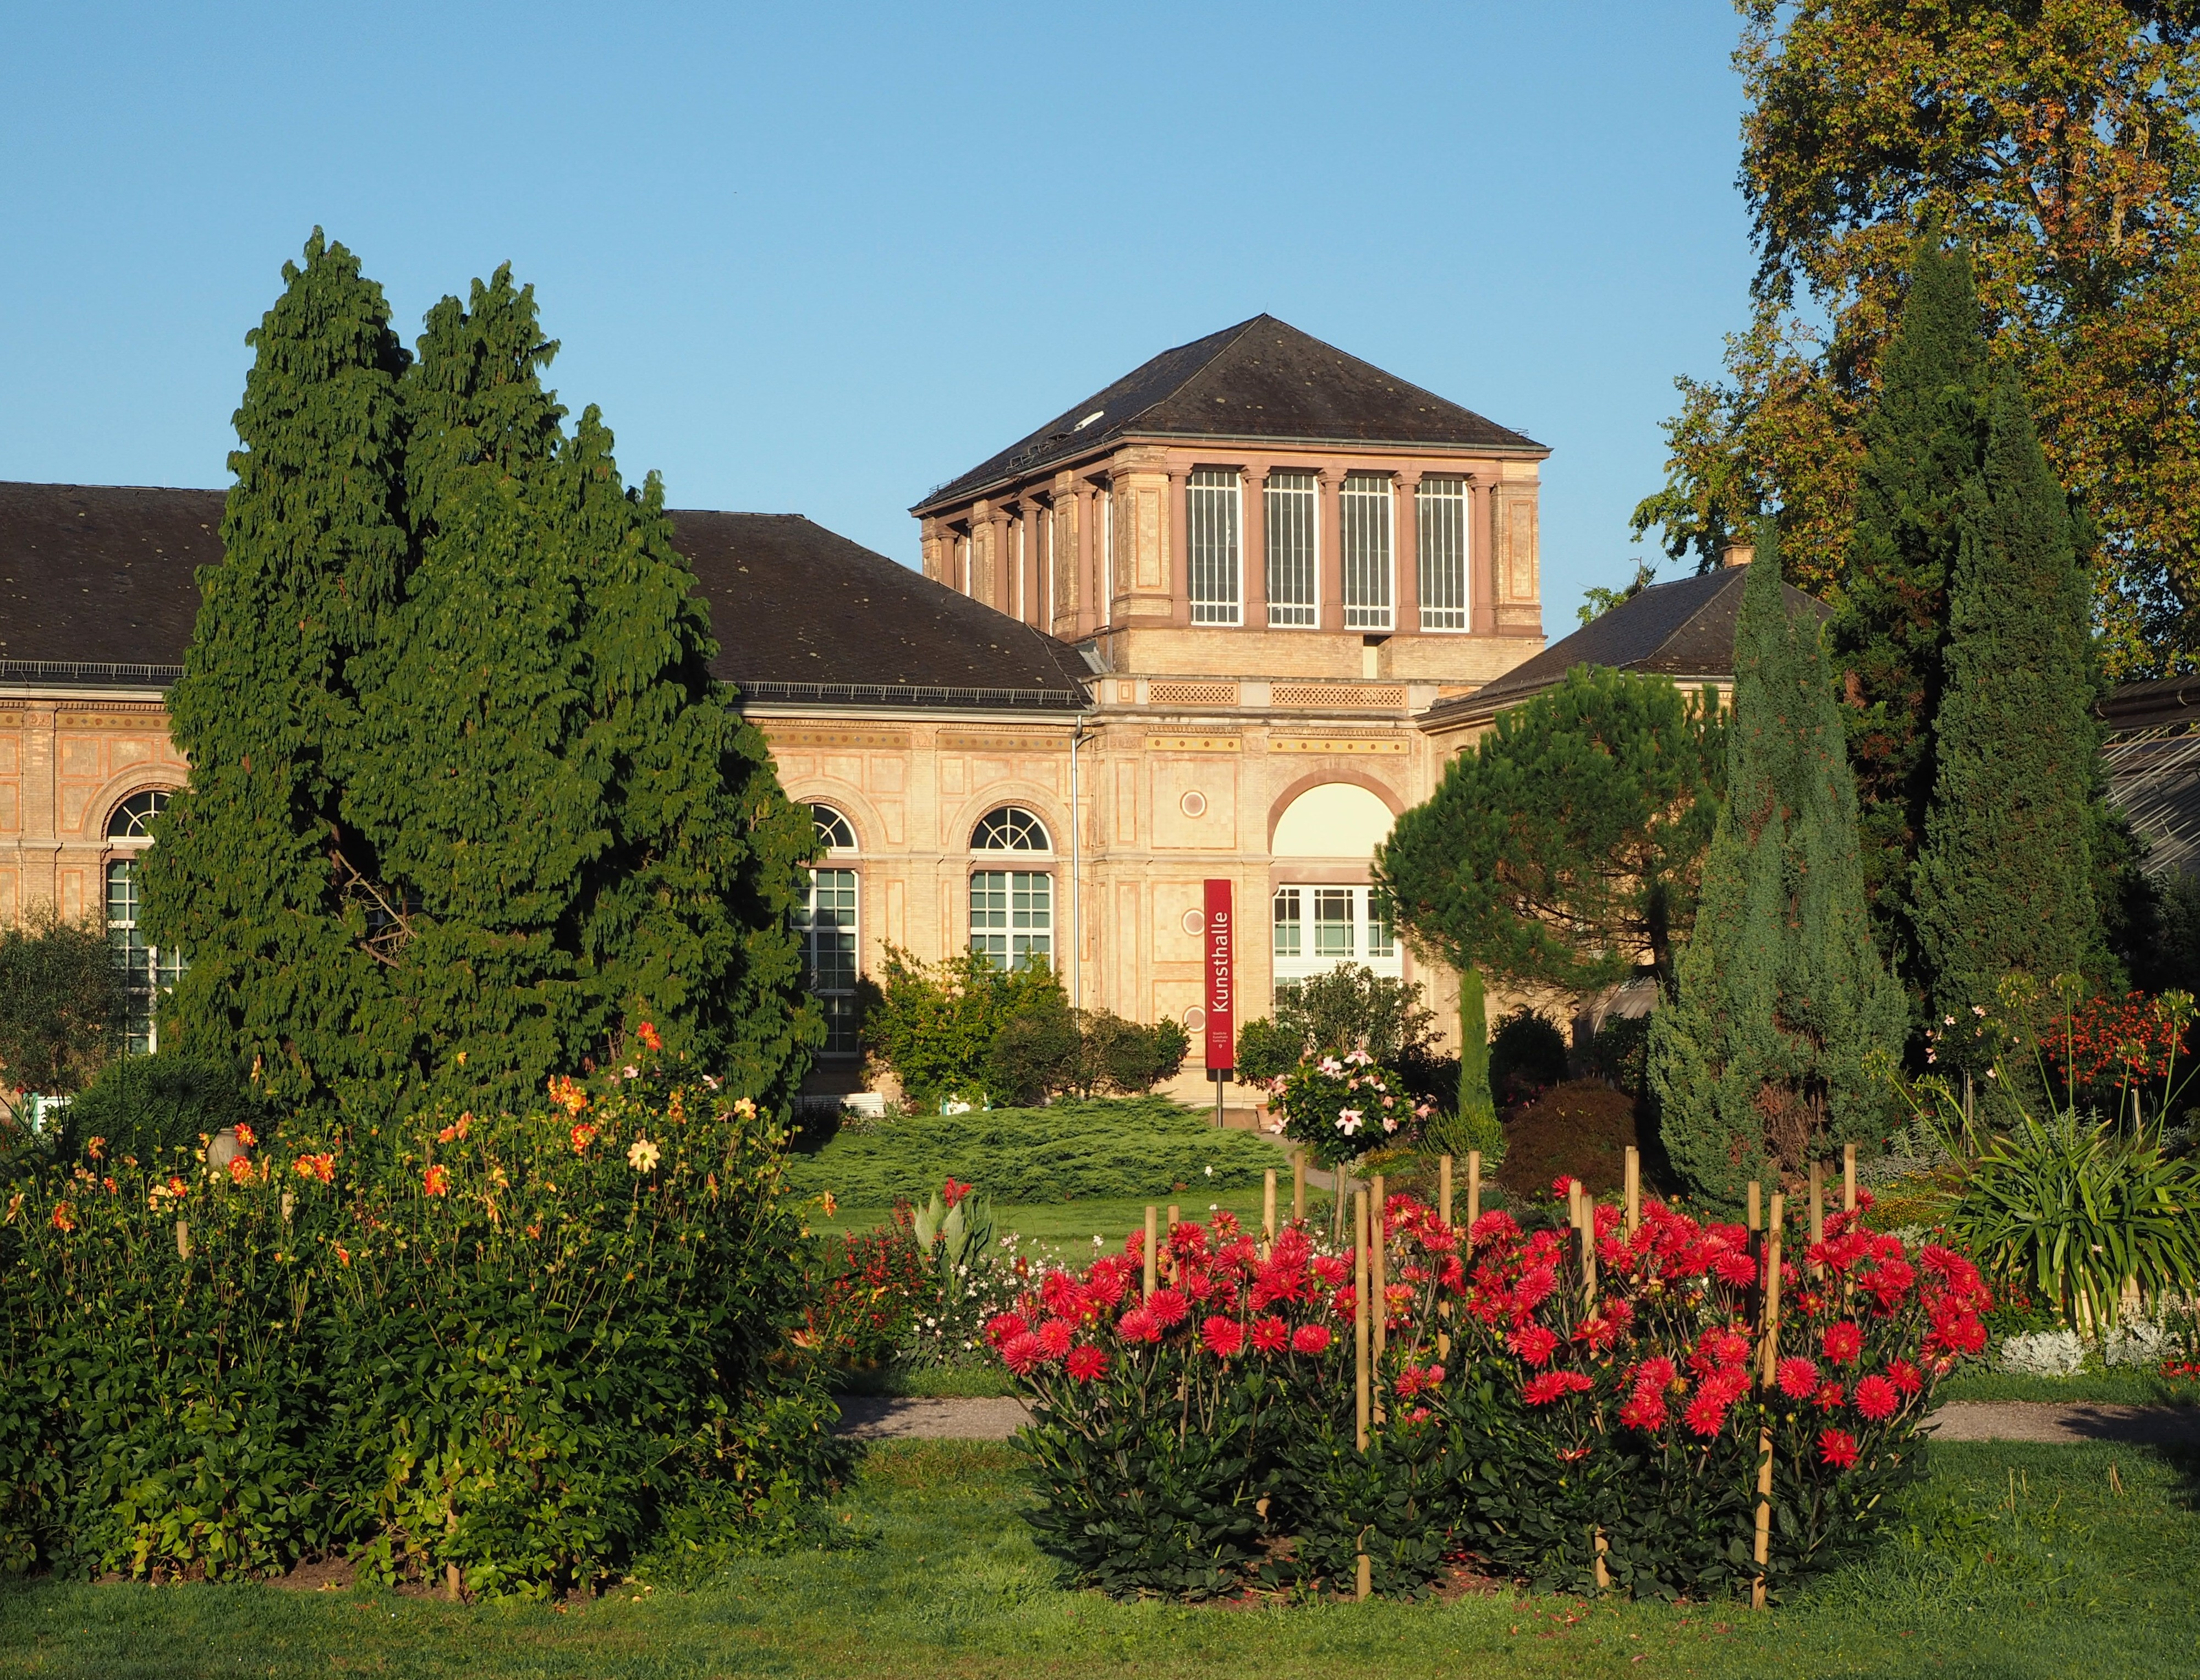
\includegraphics[width=21cm,clip,trim=0 250 0 400]{images/city/botanic-gardens-1.jpg}};
  \end{scope}
  \node[anchor=south west,color=black,xshift=1ex,yshift=1ex] (label) at (img.south west) {\imgtitle{Benjamin Berg}{Botanic Garden and Art Galery}{CC BY-SA 4.0}};
  \begin{scope}[on background layer]
    \node[fit=(label),inner sep=0,outer sep=0,opacity=0.6,fill=white,rounded corners] {};
  \end{scope}
\end{tikzpicture}

\vspace*{8.8cm}

\section{Sponsors}

This section describes how we envision to raise the money needed for running the event.

Karlsruhe is not only a student city; it is also a hub for IT companies. Every year, events such as LEARNTEC and initiatives such as KAIT-SI or MEKA are hosted in Karlsruhe, bringing together professionals from the area of security, mobile computing and design.
We believe that hosting GUADEC 2016 in Karlsruhe can contribute to anchoring GNOME in a sustainable way in the wider network of a fast-growing IT-cluster in Germany which has its central point in Baden-Württemberg.
We further commit to closely interact with the local government, administration and tourism board to ensure that as many entities as possible are aware of the unique opportunity that an event such as GUADEC is providing to members of the GNOME community, but also to the wider public.  

We intend to produce a sponsorship brochure which shows the value GUADEC and GNOME adds.
In that brochure, we intend to have several sponsorship packages which include the usual perks such as a logo on the conference banner, the booklet and website.
In addition we reserve the opportunity to sponsor single 

We intend to contact various IT companies in the region, for example SAP, Web.de, secorvo, 
%http://www.techpark.de/tpk/inhalt/nav/der-technologiepark/unternehmen-im-tpk/uebersicht.xml?ceid=115085&dyn=true
CAS, Gameforge, B2M, 
% http://www.cyberforum.de/mitglieder/unsere-mitglieder/mitglieder-von-a-z/
% http://www.ka-it-si.de/partner/index.html
Sophos, Wibu,
and others.


As per the budget shown below, we might rely on money we will not acquire ourselves.
